\documentclass[a4paper,11pt]{article}
\usepackage{a4wide}
\usepackage{fullpage}
\usepackage[utf8x]{inputenc}

\usepackage[light,math]{anttor}
\usepackage[T1]{fontenc}

%\usepackage[slovene]{babel}
%\selectlanguage{slovene}
\usepackage[toc,page]{appendix}
\usepackage[pdftex]{graphicx} 

\usepackage{lmodern}
\usepackage{amsmath}
\usepackage{amssymb}
\usepackage{amsthm}
\usepackage{amsfonts}
\usepackage{mathtools}
\usepackage{enumitem}
\usepackage{amsfonts}
\usepackage{amsmath}
\usepackage{setspace}
\usepackage{color}
\definecolor{light-gray}{gray}{0.95}
\usepackage{listings} 
\usepackage{hyperref}
\renewcommand{\baselinestretch}{1.2} 
\renewcommand{\appendixpagename}{Priloge}


\title{ Detecting contours of human organs in CT images \\ 
using the Canny edge detector }
\author{Sara Bizjak}
\date{\today}

%%%%%%%%%%%%%%%%%%%%%%%%%%%%%%%%%%%%%%%%%%%%%%%%%%%%%%%%%%%%%%%%%%%%%%%%%%%%%%%%%%%%%%%%%%%%%%%%%%%%%%%%%%%%%%%%%%%%%%%%%%%%%%%%%

\begin{document}

\maketitle

\begin{center}
\section*{Abstract}
\end{center}
This paper represents results of detecting contours of human organs in the CT images from the DTMRI DB (\cite{bib:db}) using the Canny edge detector.
%%%%%%%%%%%%%%%%%%%%%%%%%%%%%%%%%%%%%%%%%%%%%%%%%%%%%%%%%%%%%%%%%%%%%%%%%%%%%%%%%%%%%%

\section{Introduction}

Edge detection is one of the most commonly used operations in image analysis. 
An edge can be defined by a discountinuity in gray level values. We could say that an edge is the boundary between the object and the background. 
Some of the most popular edge detecting algorithms are Marr-Hildreth, Canny edge, the local threshold and boolean function based edge detector and others.
For our analysis we used Canny edge detector.


%%%%%%%%%%%%%%%%%%%%%%%%%%%%%%%%%%%%%%%%%%%%%%%%%%%%%%%%%%%%%%%%%%%%%%%%%%%%%%%%%%%%%%

\section{Methodology}

%%%%%%%%%%%%%%%%%%%%%%%%%%%%%%%%%%%%%%%%%%%

\subsection{Terms}

\textbf{The Canny edge detector} is an algorithm to detect contour on images, in our case, to detect contours of human organs in CT images.
Basic steps of the Canny edge detection algorithm:
\begin{enumerate}
    \item Smooth the input image with Gaussian filter
    \item Compute the gradient magnitude and angle images
    \item Apply nonmaxima suppression to the gradient magnitude image
    \item Use double thresholding and connectivity analysis to detect and link edges
\end{enumerate}

\noindent
\textbf{Gaussian filter} is a smoothing spatial filter. It is used for rearranging intensities in inage with the aim to smooth sharp peaks.
One way to smooth the images is to calculate averages of surroundings for every pixel and replace that pixel with averaged value. 
The Gaussian filter works on similar principle, except that the average is weighted. 
That means that the pixel we are calculating value for has the largest weight (it is considered the most important in this calculation)
and the further we go from that pixel, the smaller impact other pixels' values have.
\\
The Gaussian function in 2-dimensions is defined as:
$$ 
G(x, y) = \frac{1}{2 \pi \sigma ^2} \cdot e^{- \frac{(x^2 + y^2)}{2 \sigma ^2}} 
$$
\begin{figure}[ht!]
    \centering
    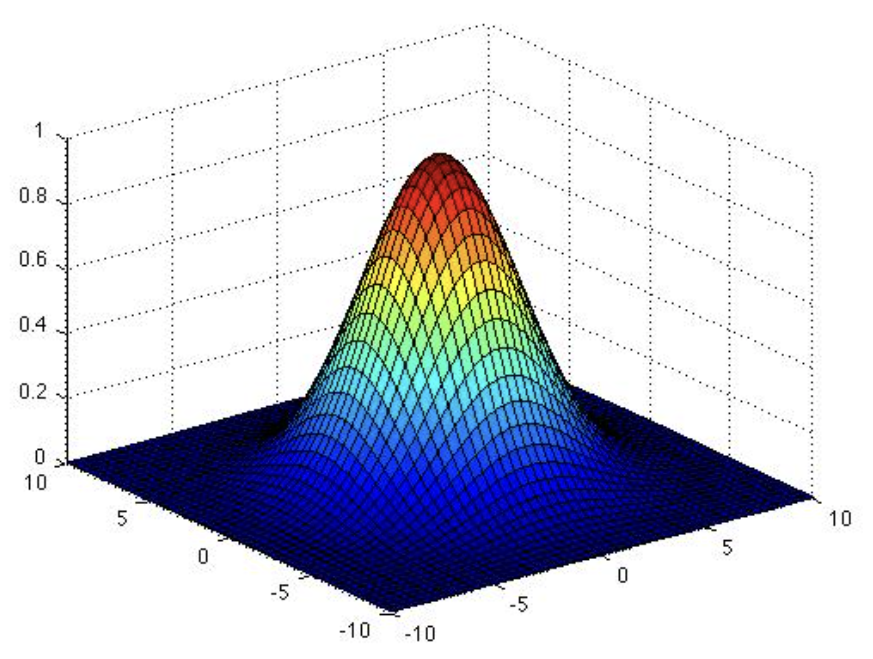
\includegraphics[width=120mm]{gaussian_filter.png}
    \caption{The two-dimensional Gaussian filter visualization.}
    \label{pic:gauss}
\end{figure}
\noindent
Since we are not in continuous space, we would like to get matrix of values (discrete values of pixels) from the equation for the Gaussian function above.
That matrix, we call it kernel, is then applied to every pixel to filter the whole image (the visualization of that matrix is similar to the figure \ref{pic:gauss}).
The kernel size (determined by parameter $\sigma$) depends on the image size.
\\
\\
\textbf{Gradient magnitude and angle images} is calculated from the first derivate of a Gaussian function.
Let $f(x,y)$ denote the input image and $G(x,y)$ denote the Gaussian function. 
The gradient is the tool of choice for finding edge strength and direction at location $(x,y)$ of an image $f(x,y)$ and it is defined as the vector 
$[g_x; gy_]$ ($g_x$ and $g_y$ are the gradients along the horizontal axis and along the vertical axis, respectively, or along two perpendicular axes). 
The magnitude of the gradient vector is defined as the vector length while the direction $\alpha(x,y)$ is given by the angle of the gradient vector with respect to the horizontal axis:
$$
M(x, y) = \sqrt{g_x^2(x, y) + g_y^2(x, y)}
$$
$$
\alpha(x, y) = \text{tg}^{-1} \left( \frac{g_y(x, y)}{g_x(x, y)} \right)
$$
There are several \textit{masks} to compute the gradient. Let us mention the three from the lectures:
\\
\\
\begin{minipage}{0.2\textwidth}
    \centering
    \textbf{Roberts:}
\end{minipage}\hfill
\begin{minipage}{0.3\textwidth}
    \begin{equation*}
        k_x = 
        \begin{bmatrix}
        -1 & 0  \\
        0 & 1 \\
        \end{bmatrix}
    \end{equation*}
    \\
\end{minipage}\hfill
\begin{minipage}{0.4\textwidth}
    \begin{equation*}
        k_y = 
        \begin{bmatrix}
        0 & -1 \\
        1 & 0 \\
        \end{bmatrix}
    \end{equation*}
    \\
\end{minipage}\hfill

\noindent
\begin{minipage}{0.2\textwidth}
    \centering
    \textbf{Prewitt:}
\end{minipage}\hfill
\begin{minipage}{0.4\textwidth}
    \begin{equation*}
        k_x = 
        \begin{bmatrix}
        -1 & -1 & -1 \\
        0 & 0 & 0 \\
        1 & 1 & 1
        \end{bmatrix}
    \end{equation*}
    \\
\end{minipage}\hfill
\begin{minipage}{0.4\textwidth}
    \begin{equation*}
        k_y = 
        \begin{bmatrix}
        -1 & 0 & 1 \\
        -1 & 0 & 1 \\
        -1 & 0 & 1
        \end{bmatrix}
    \end{equation*}
    \\
\end{minipage}\hfill
\begin{minipage}{0.4\textwidth}
\end{minipage}\hfill

\noindent
\begin{minipage}{0.2\textwidth}
    \centering
    \textbf{Sobel:}
\end{minipage}\hfill
\begin{minipage}{0.3\textwidth}
    \begin{equation*}
        k_x = 
        \begin{bmatrix}
        -1 & -2 & -1 \\
        0 & 0 & 0 \\
        1 & 2 & 1
        \end{bmatrix}
    \end{equation*}
    \\
\end{minipage}\hfill
\begin{minipage}{0.4\textwidth}
    \begin{equation*}
        k_y = 
        \begin{bmatrix}
        -1 & 0 & 1 \\
        -2 & 0 & 2 \\
        -1 & 0 & 1
        \end{bmatrix}
    \end{equation*}  
    \\
\end{minipage}\hfill


\noindent
\textbf{Non-maxima suppression} is a scheme for thinning the ridges and works as follows:
\begin{itemize}
    \item Among the four basic regions (vertical, horizontal and diagonal) find the one closest to angle $\alpha(x, y)$
    \item If the value of $M(x, y)$ (magnitude) is less than at least one of its two neighbour along delected region, then the pixel at $(x, y)$ is set to $0$. Otherwise it is set to $M(x, y)$
\end{itemize}

\noindent
\textbf{Double thresholding} is a detector for determing "safe" edges depending on pixel intensity. That means that we use two thresholds, denote them as TH and TL (high and low). 
If the intensity of a pixel is higher than TH, we say that selected pixel is definitely located on the edge. 
Similarly, if the intensity of a pixel is lower than TL, we say that selected pixel is definitely \textit{not} on the edge.
If the pixel intensity drops somewhere in between TL and TH, we cannot determine whether it is on the edge or not.
TH and TL are choosen as a proportion of the maximal intensity on the picture. 
\\
\\
\noindent
\textbf{Connectivity analysis} serves to connect the edges properly, that means that \textit{a pixel close enough to an edge is also the same edge.}
To say it more formally, we form longer edges using 8-connectivity from weak pixels to strong pixels, that is, for every pixel, we check whether the neighbours are a part of an edge. If there exists one, we connect the observed pixel to the same edge.
To make the better results, we repeat the process several times and in several directions.


%%%%%%%%%%%%%%%%%%%%%%%%%%%%%%%%%%%%%%%%%%%

\subsection{Usage}

For our algorithm, we used Gaussian filter with parameter $\sigma$ determined as 
$$
\sigma = (\text{minimal value of pixel on the image}) \cdot 0.005
$$
and Prewitt's mask. Thresholds were set as:
\begin{itemize}
    \item TH is set as $20 \%$ of maximal magnitude intensity,
    \item TL is set as $10 \%$ of maximal magnitude intensity.
\end{itemize}    
For connecting edges we used window size 1 and made multiple repetitions.
%%%%%%%%%%%%%%%%%%%%%%%%%%%%%%%%%%%%%%%%%%%%%%%%%%%%%%%%%%%%%%%%%%%%%%%%%%%%%%%%%%%%%%

\section{Results}

\subsection{Testing example}
In this section are presented results of stages for one selected image from CTMRI DB. The stages of the process are written in the images' descriptions.

\begin{figure}[ht!]
    \begin{minipage}{0.5\textwidth}
        \centering
        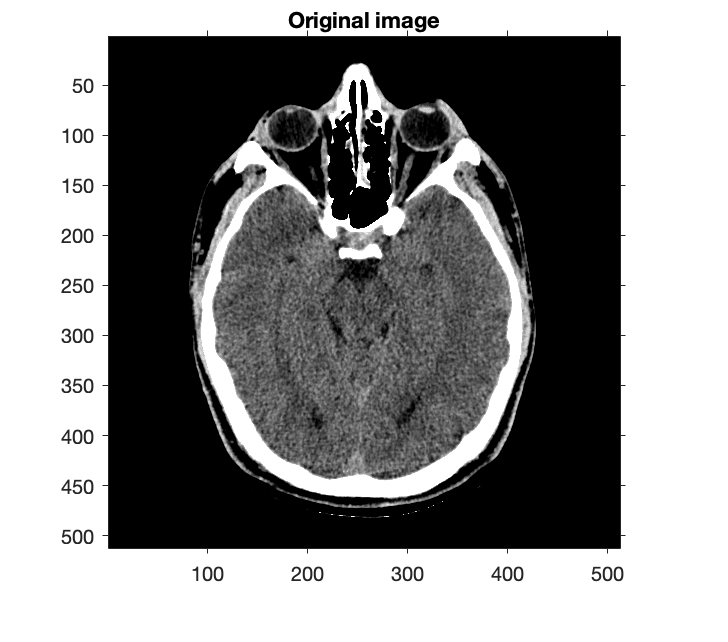
\includegraphics[width=80mm]{original.png}
        \caption{Original image.}
    \end{minipage}\hfill
    \begin{minipage}{0.5\textwidth}
        \centering
        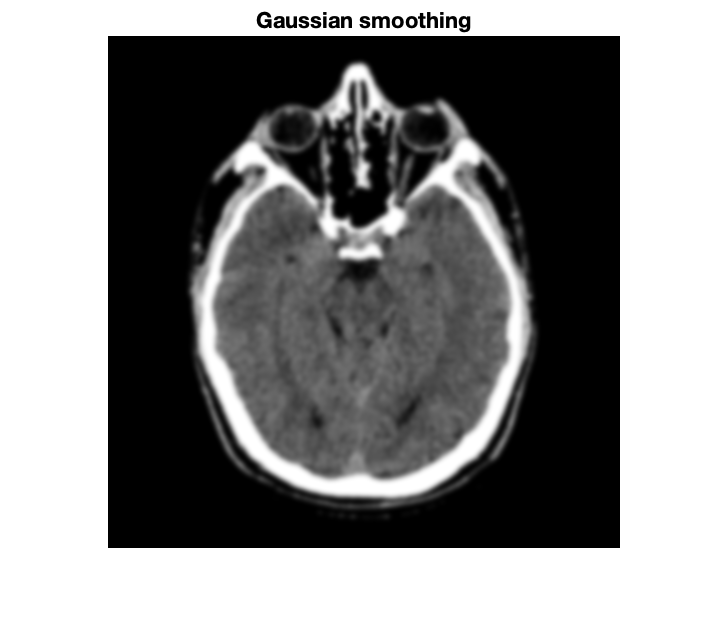
\includegraphics[width=80mm]{gauss.png}
        \caption{Image after Gaussian smoothing.}
    \end{minipage}\hfill
\end{figure}
\noindent
\begin{figure}[ht!]
    \begin{minipage}{0.5\textwidth}
        \centering
        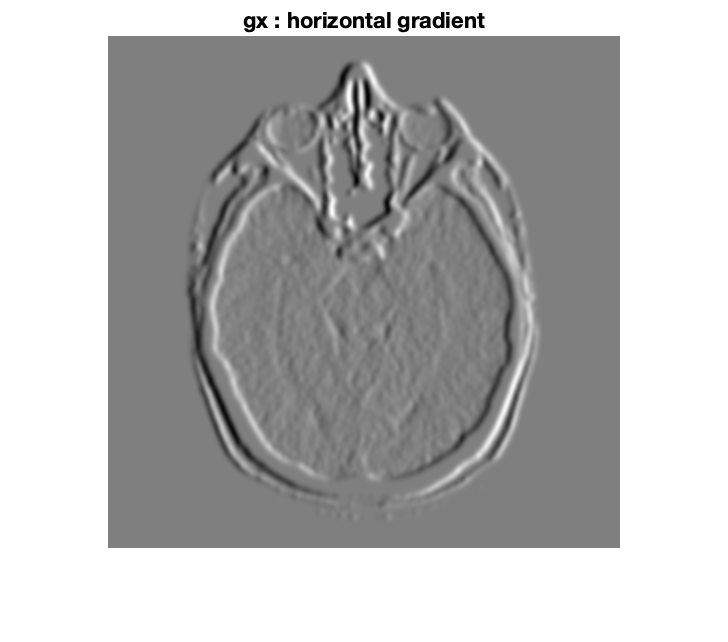
\includegraphics[width=60mm]{gx.png}
        \caption{Horisontal gradient visualization.}
    \end{minipage}\hfill
    \begin{minipage}{0.5\textwidth}
        \centering
        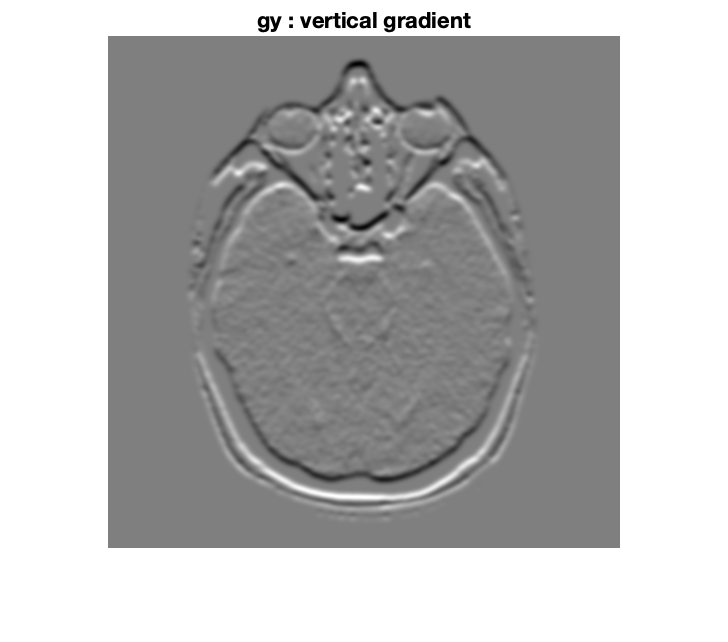
\includegraphics[width=60mm]{gy.png}
        \caption{Vertical gradient visualization.}
    \end{minipage}\hfill
\end{figure}
\noindent
\begin{figure}[ht!]
    \begin{minipage}{0.5\textwidth}
        \centering
        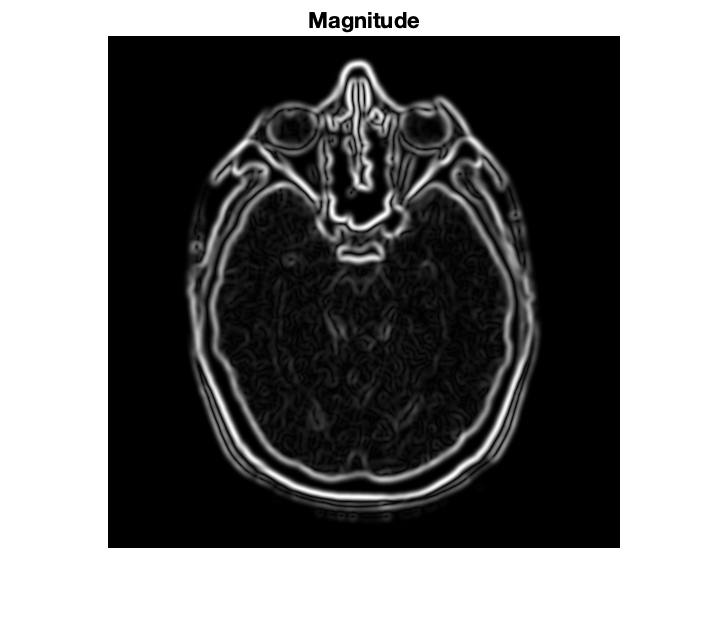
\includegraphics[width=80mm]{magnitude.png}
        \caption{Magnitude visualization.}
    \end{minipage}\hfill
    \begin{minipage}{0.5\textwidth}
        \centering
        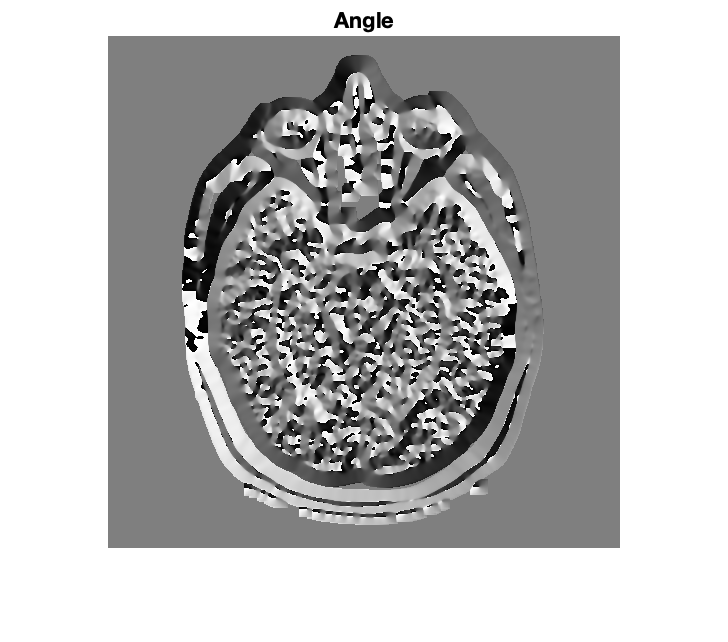
\includegraphics[width=80mm]{angle.png}
        \caption{Angle visualization.}
    \end{minipage}\hfill
\end{figure}
\noindent
\begin{figure}[ht!]
        \centering
        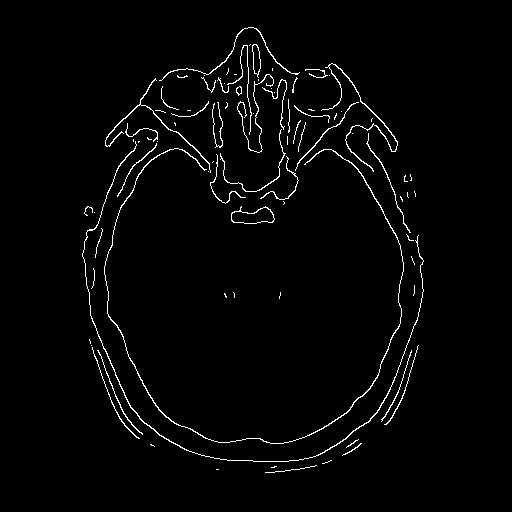
\includegraphics[width=90mm]{canny_edge.png}
        \caption{Image after canny edge detection.}
\end{figure}

\newpage
\noindent
For further analysis, or rather, for an attempt to improve the result of the algorithm, 
we try the Poisson smoothing filter (source \cite{bib:poiss}) that generates the Poisson noise from the data.
The result of edge detecting can be better, but we must set the TH and TL by hand empirically.
For the same image as above, the TH and TL were calculated as (we also increase TL so the relationship between TH and TL remains the same):
\begin{itemize}
    \item TH is set as $28 \%$ of maximal magnitude intensity,
    \item TL is set as $18\%$ of maximal magnitude intensity.
\end{itemize}  
Take a look at the image after canny edge detection with Poisson smoothing filter:
\begin{figure}[ht!]
    \centering
    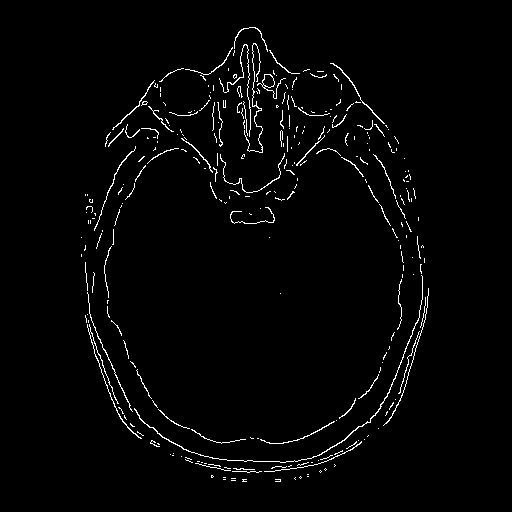
\includegraphics[width=90mm]{0090_poisson.png}
    \caption{Image after canny edge detection using Poisson smoothing filter.}
\end{figure}

\subsection{Other examples}
In this section are presented some other examples (original image and image after canny edge detection). 
In canny edge algorithm we used different parameters (starting with our standard $20 \%$ and $10 \%$ for TH and TL and then change them manualy) and different smoothing filters -- depends on which parameters and filter achieved better results.

\begin{figure}[ht!]
    \begin{minipage}{0.5\textwidth}
        \centering
        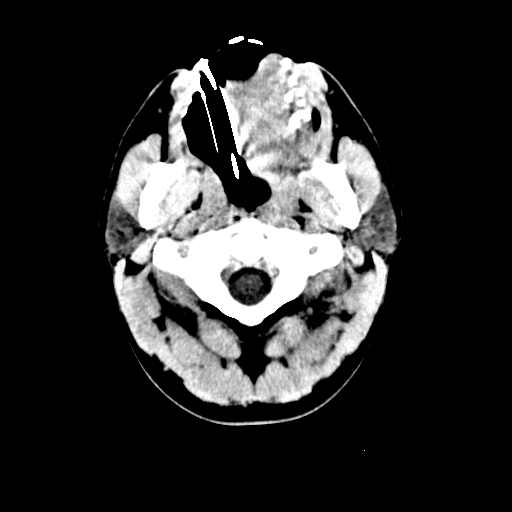
\includegraphics[width=55mm]{0001.png}
        \caption{Original image.}
    \end{minipage}\hfill
    \begin{minipage}{0.5\textwidth}
        \centering
        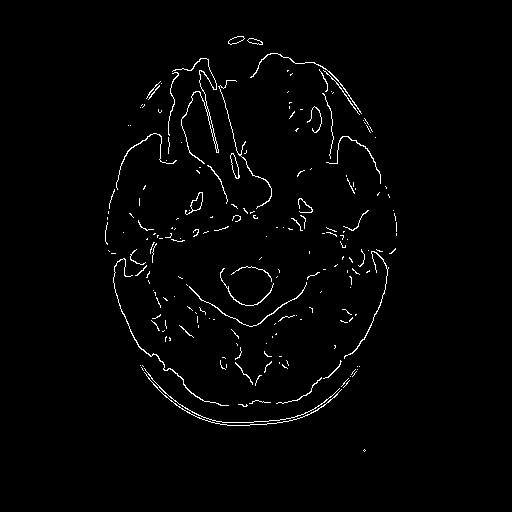
\includegraphics[width=55mm]{0001_poisson.png}
        \caption{Image after canny edge detection using Poisson smoothing.}
    \end{minipage}\hfill
\end{figure}

\noindent
\begin{figure}[ht!]
    \begin{minipage}{0.5\textwidth}
        \centering
        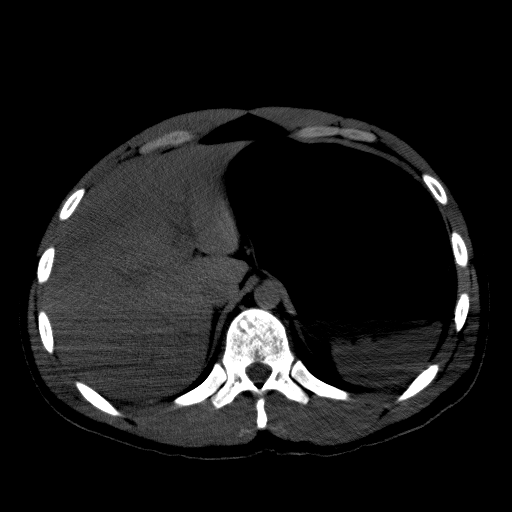
\includegraphics[width=55mm]{0005.png}
        \caption{Original image.}
    \end{minipage}\hfill
    \begin{minipage}{0.5\textwidth}
        \centering
        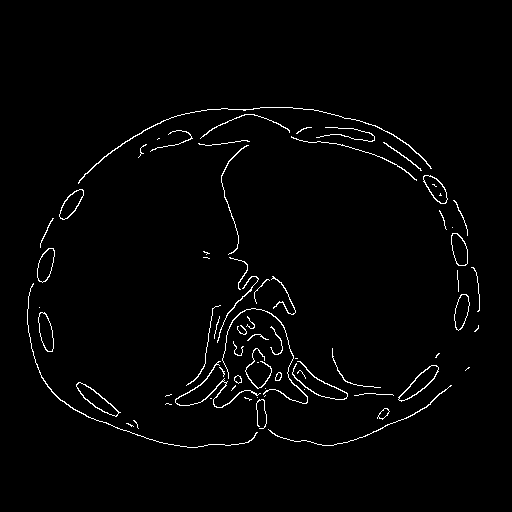
\includegraphics[width=55mm]{0005_canny.png}
        \caption{Image after canny edge detection using Gaussian smoothing.}
    \end{minipage}\hfill
\end{figure}

\noindent
\begin{figure}[ht!]
    \begin{minipage}{0.5\textwidth}
        \centering
        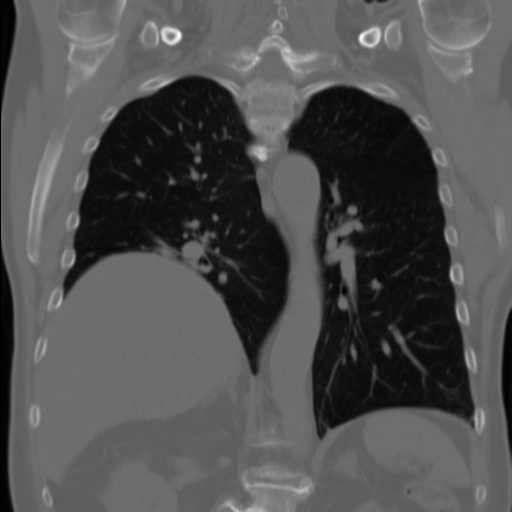
\includegraphics[width=55mm]{0015.png}
        \caption{Original image.}
    \end{minipage}\hfill
    \begin{minipage}{0.5\textwidth}
        \centering
        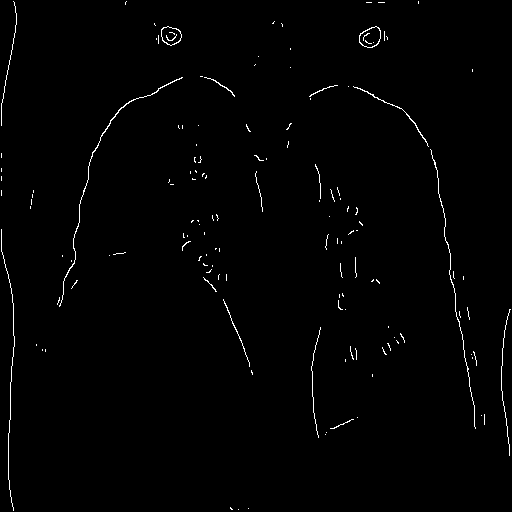
\includegraphics[width=55mm]{0015_poisson.png}
        \caption{Image after canny edge detection using Poisson smoothing.}
    \end{minipage}\hfill
\end{figure}

\noindent
\begin{figure}[ht!]
    \begin{minipage}{0.5\textwidth}
        \centering
        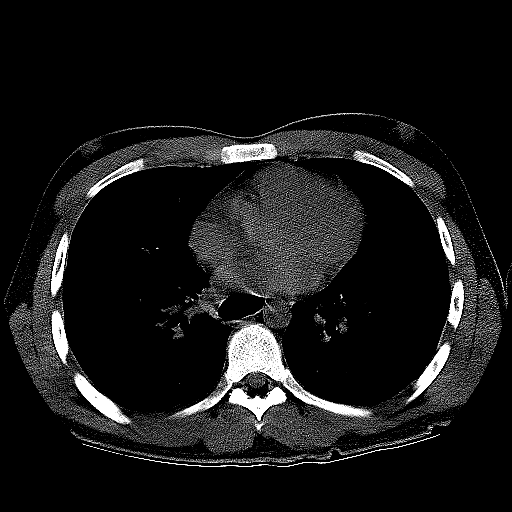
\includegraphics[width=55mm]{0020.png}
        \caption{Original image.}
    \end{minipage}\hfill
    \begin{minipage}{0.5\textwidth}
        \centering
        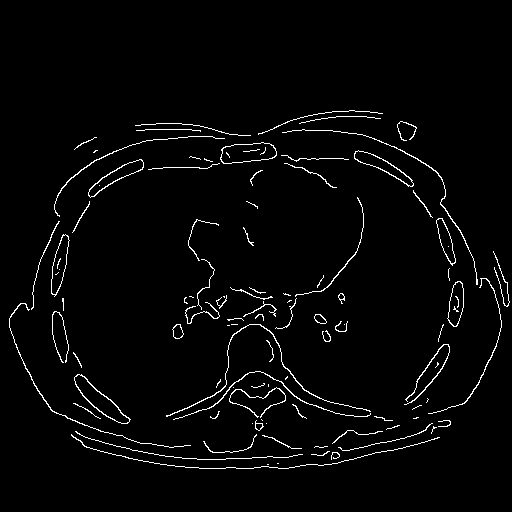
\includegraphics[width=55mm]{0020_canny.png}
        \caption{Image after canny edge detection using Gaussian smoothing.}
    \end{minipage}\hfill
\end{figure}

\newpage
\noindent
\begin{figure}[ht!]
    \begin{minipage}{0.5\textwidth}
        \centering
        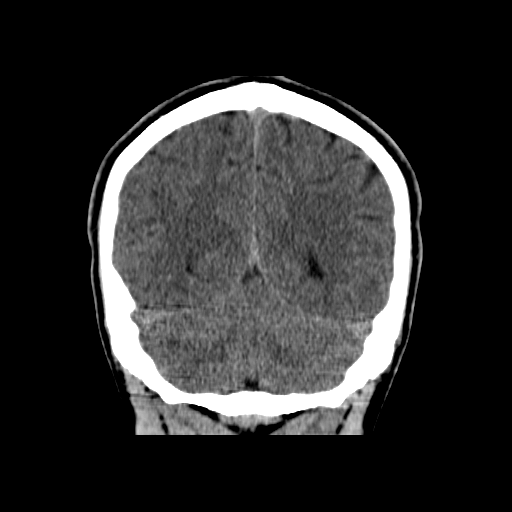
\includegraphics[width=55mm]{0080.png}
        \caption{Original image.}
    \end{minipage}\hfill
    \begin{minipage}{0.5\textwidth}
        \centering
        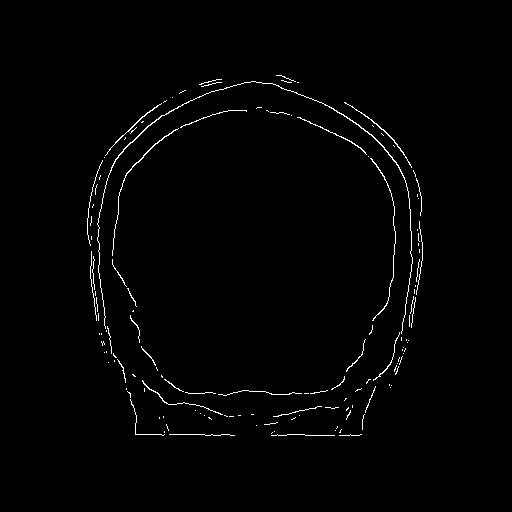
\includegraphics[width=55mm]{0080_poisson.png}
        \caption{Image after canny edge detection using Poisson smoothing.}
    \end{minipage}\hfill
\end{figure}

%%%%%%%%%%%%%%%%%%%%%%%%%%%%%%%%%%%%%%%%%%%%%%%%%%%%%%%%%%%%%%%%%%%%%%%%%%%%%%%%%%%%%%


\section{Conclusion}
The results of our canny edge algorithm are satisfactory.
Our selected threshold (TH as $20 \%$ and TL as $10 \%$ of maximal magnitude intensity) works fine in general,
but to improve results of the algorithm, it is better to calibrate the parameters for each image separately, since they can vary a little.
However, it is important that TH and TL remain in the similar relationship, that is, 
that proportion of intensity for which we cannot determine if the pixel is an edge or not (the intensity between TH and TL) is always about the same.
Also, for every image we can determine which smoothing filter (Gaussian or Poisson) works better and perform canny edge with the better filter.


%%%%%%%%%%%%%%%%%%%%%%%%%%%%%%%%%%%%%%%%%%%%%%%%%%%%%%%%%%%%%%%%%%%%%%%%%%%%%%%%%%%%%%

\begin{thebibliography}{99}
    \bibitem{bib:db}
    \emph{DTMRI DB}, [viewed 6.~1.~2021], available at \url{http://lbcsi.fri.uni-lj.si/OBSS/Data/CTMRI/}.
    
    \bibitem{bib:poiss}
    \emph{Poisson smoothing filter}, [viewed 6.~1.~2021], \url{https://www.mathworks.com/help/images/ref/imnoise.html}.


\end{thebibliography}

\end{document}